
\section{Introduction} 
\label{sec: intro}

The scale of supercomputers continually grows at a breakneck pace to 
accommodate the computing power requirements for scientific research. 
Supercomputers have tens of thousands of nodes and serve as an irreplaceable 
research vehicle for scientific problems with increasing size and complexity. 
Supercomputers are usually employed as a shared resource to 
accommodate many parallel applications (jobs) running concurrently. 
These parallel jobs share the system infrastructure such as network and I/O bandwidth, 
and inevitably there is contention over these shared resources. 
As supercomputers continue to evolve, these shared resources are increasingly the bottleneck for performance.


\begin{figure}[h!]
    \centering
    \begin{subfigure}[t]{0.22\textwidth}
        \centering
        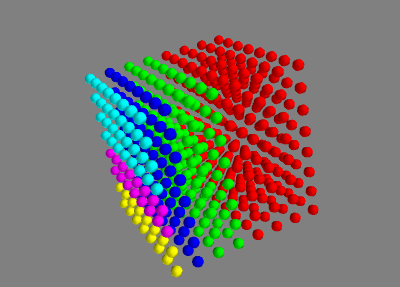
\includegraphics[height=1.2in]{figs/goodallocation}
        \caption{Contiguous}
        \label{fig:overview_sub1}
    \end{subfigure}%
    \hspace{1em}%
    \begin{subfigure}[t]{0.22\textwidth}
        \centering
        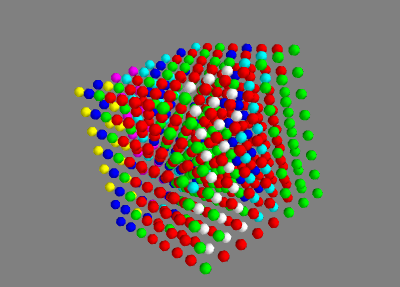
\includegraphics[height=1.2in]{figs/badallocation}
        \caption{Non-contiguous}
        \label{fig:overview_sub2}
    \end{subfigure}%
   \caption{Multiple jobs running concurrently with different allocations. 
   Each job is represented by a specific color. 
   a) shows the effect of contiguous job placement, 
   which could possibly reduce the inter-job interference. 
   b) shows non-contiguous job placement, 
   which may introduce both intra and inter-job interference. 
   }
   \label{fig:overview}
\end{figure}

When submitting jobs to HPC systems, 
users request system resources by specifying the number of compute nodes and expected runtime. 
The batch scheduler is then responsible for dispatching the submitted jobs to the system. 
Typically, there are multiple jobs running concurrently on the system,
resulting in the shared use of resources, particularly network links. 
A prominent problem with this network sharing is the contention over
the network among those concurrently running jobs. 
The network contention can cause communication variability and 
performance degradation to those jobs~\cite{abhinav-sc13}. 
This performance degradation can propagate into the queueing time of the following submitted jobs, 
thus leading to low system throughput and utilization~\cite{jose-ipdps15}. 
This adverse effect of network sharing can be mitigated by 
providing jobs with isolated allocations and exclusive network resources.

On the widely used torus-connected HPC systems~\cite{bgq,tofu,titan}, 
two job placement policies are commonly used. 
In \emph{contiguous placement} policy, 
each job gets a compact and contiguous set of computing nodes, 
as shown in Figure~\ref{fig:overview_sub1}. 
The partition-based placement adopted on the Blue Gene 
series systems is an example of contiguous placement policy~\cite{bgloverview}. 
The contiguous placement favors application performance 
through exclusive networking within a compact partition 
and the locality that implies. 
However, contiguous placement can cause both internal fragmentation 
(when more nodes are allocated to a job than it requests) 
and external fragmentation 
(when sufficient nodes are available for a request, but they can not be allocated contiguously), 
therefore leading to lower system utilization than is otherwise possible. 
On the other hand, the \emph{non-contiguous placement} policy, 
adopted by the Cray XT/XE series~\cite{carl-cug}, 
assigns free nodes to jobs regardless of contiguity, 
though of course efforts are made to maximize locality. 
Figure~\ref{fig:overview_sub2} shows the effect of non-contiguous placement. 
While eliminating internal and external fragmentation as seen in contiguous placement systems, 
in return non-contiguous placement policy introduces contention between jobs due to the interleaving of job nodes. 
The non-contiguous job placement can significantly reduce job performance, 
especially for communication-intensive ones~\cite{abhinav-sc13}.

We envision that future HPC systems will be equipped with 
a flexible job placement mechanism which combines the 
best of both contiguous and non-contiguous policy. 
Such a flexible job placement mechanism should take 
shared resource needs (e.g., network resources) of jobs into account 
when making scheduling and allocation decisions. 
With the knowledge and analysis of job communication patterns, 
it can be identified which jobs require exclusive network and compact allocation, and to what degree. 
Then, rather than allocating each job in a ``know-nothing'' manner, 
one may specialize job placement policy so that, for example, 
only the jobs with stringent network needs are given compact, isolated allocations, 
resulting in maximized utilization and minimized perceivable resource contention effects.

In this work, we focus on an in-depth analysis of intra- and inter-job 
communication interference with different job placements on torus-connected HPC systems. 
Torus-based networks are used on six of the top 10 supercomputers 
on the June 2015 Top500 lists~\cite{top500}. 
The current generation of IBM Blue Gene/Q (BG/Q) supercomputers, 
such as Mira at Argonne Nation Laboratory and 
Sequoia at Lawrence Livermore National Laboratory, 
have their compute nodes connected by a 5D torus network~\cite{bgq}. 
The K computer from Japan uses the ``Tofu'' interconnected system, 
which has a 6D mesh/torus topology~\cite{tofu}. 
Titan, a Cray XK7 supercomputer located at the Oak Ridge Leadership Computing Facility (OLCF), 
has nodes connected in a 3D torus within the compute partition~\cite{titan}. 
Although our analyses are based on torus networks, 
the ideas conveyed in this work is applicable to networks with different topologies. 

We selected three signature applications from 
the DOE Design Forward Project~\cite{designforwardwebpage} as examples 
to conduct detailed study about the communication pattern of parallel applications. 
We use a sophisticated simulation toolkit named CODES 
(standing for Co-Design of Multi-layer Exascale Storage Architectures)~\cite{Jason-2011} 
as a research vehicle to evaluate the performance of these applications 
with various allocations in a controlled environment. 
We then analyze the intra- and inter-job interference 
by simulating these applications running concurrently with different allocations. 
We believe the insights presented in this work can be very useful 
for the design of future HPC batch schedulers and resource managers.


The rest of this paper is organized as follows. 
Section~\ref{sec:application study} describes the three representative applications 
from the DOE Design Forward Project for our study. 
Section~\ref{sec:codes} talks about the use of CODES as research vehicle for our work. 
%Section~\ref{sec:config study} shows the performance analysis of three applications on different torus networks. 
Section~\ref{sec:interference} provides detailed analysis about the intra- and inter-job interference 
among three applications on torus network with different allocations. 
Section~\ref{sec:discussion} introduces a path toward communication-pattern aware allocation strategies, 
given the results of our analysis. 
Section~\ref{sec:related_work} discusses related work. 
Finally, the conclusion is presented in Section~\ref{sec:conclusion}.




